\documentclass[11pt,letterpaper]{article}
\usepackage[latin1]{inputenc}
\usepackage{amsmath}
\usepackage{amsfonts}
\usepackage{amssymb}
\usepackage{graphicx}
\usepackage[left=1.00in, right=1.00in, top=1.00in, bottom=1.00in]{geometry}
\usepackage{hyperref}
\author{Andrew Rosen, Brendan Benshoof, Anu G. Bourgeois, Robert W. Harrison}
\date{}
\title{How to Build Distributed Governed Systems}
\begin{document}
	\maketitle
	
	
	Developers and researchers typically use one of two models when building a distributed system.
	The first is a completely centralized model, where one server or person is in control.
	The other alternative is a completely decentralized model, where no single entity has control, except for perhaps the protocol itself.
	
	In practice, this is not the only models that exist in the wild.  
	
	How can we create a system that balances multiple powerful entities against each other?
	
	


	Nomic is a game created by Peter Suber in 1982 \cite{nomic}.
	The initial rules of the game define a goal (gaining points) and describe how Nomic works.
	Each ``move'' in the game is a proposition to add, remove, or amend the rules of the game (unless of course, the rules have defined new actions that players can take for their turns).
	Any modification to the rules is then voted upon by the players and goes into effect (again, unless the rules have moved the system away from a democracy).
	The player then collects points.
	
	Previous work has been done on using Nomic as the system for blockchain based systems for Bitcoin or other cryptocurrencies \cite{tezos} using a constructed language.
	We want to show how Nomic can be used as the basis for building a wide variety self-governing distributed systems from blockchains, to administrating servers, to solving very interesting problems in managing DNS and security, such as key revocation.
	Governomic also does not assume the need for a constructed language.
	
	
	\subsection{Types of Governments}
	Because Nomic is a system for laying down rules, defining who can do what and who has power, we can use it to simulate just about any form of governmental system implemented by humans. 
	Some examples:
	\begin{itemize}
		\item An autocracy, a system where power and authority is vested in a single entity. 
		\item An aristocracy, where only chosen members of the system get to vote, or even have a voice.
		\item A plutocracy, where a large sum of currency is needed to either participate or take an action. In other words, he who has the gold makes the rules.
		\item A representative democracy, where users in the system collectively appoint individuals to act as their proxy or proxies.
		\item A pure democracy, where each users can or must vote on each issue.
	\end{itemize}
	
	There are many variations that can be taken from history.  
	For example, a representative democracy might elect to temporarily appoint a dictator with a wide range of powers, but limited in certain capacities, much like the Roman dictator and general Lucius Quinctius Cincinnatus.
	There are number of methods that would be impractical  in a non-computing  environment, but can be managed here, such as choosing a new dictator every 5 minutes.
	
	
	\subsection{This Sounds Like How a Blockchain works, so why not that?}
	
%	The concept of a Blockchain comes from Bitcoin.
%	Bitcoin's blockchain is essentially a shared ledger.  
%	The blockchain (Figure \ref{fig:blockchain}) acts as a record of all Bitcoin transactions. 
%	Each transaction refers to a previous transaction, which indicates the funds belong to who the transactions says they do. 
%	Validation of the record is accomplished by traversing the tree of transactions and marking the referenced transactions as used. 

	Bitcoin's blockchain is essentially a shared ledger.  The blockchain (Figure \ref{fig:blockchain}) is a record of every single transaction made using the Bitcoin. Each transaction refers to  a previous transaction, indicating the funds handled by the new transaction are in fact owned by the user initiating the transaction. The record is validated by traversing the tree of transactions and marking the referenced transactions as used. A valid blockchain has all non-leaf node transactions marked as used only once.
	
	\begin{figure}
		\centering
		\includegraphics[width=0.75\linewidth]{figs/blockchain}
		\caption{A section of the blockchain as defined by Bitcoin \cite{bitcoin}.}
		\label{fig:blockchain}
	\end{figure}
	
	
	
	Transactions are grouped together and verified in a \emph{block}, which are linked together in a chain.  
	Each block in the chain is a series of transactions published during the time it takes to generate that block. 
	The process of authenticating these transactions and generating a new block is called mining.  
	Mining a block is analogous to the concept of gold mining, as the incentive for successfully mining a block is a large sum of new bitcoins.  
	
	
	Blockchains have proven to be an interesting solution and been implemented with success in the now famous Bitcoin protocol.
	However, the proof-of-work is not optimal for many uses cases, due to the amount of energy it uses and the ever increasing hardware race involved in ``mining'' blocks (Figure \ref{fig:speed-lin}).
	
	
	
	This increase in computational power is due to the way proof-of-work is done in Bitcoin.  
	In order to mine a new block and create new bitcoins, a user must generate a hash using the hash of the previous block, new transactions, and a nonce.  
	The more hashes are performed over the entire system,  the quicker the Bitcoin network will mine blocks. 
	Likewise, the more hashes an individual can perform, the better their chances of claiming the block and creating new Bitcoins (a block is worth roughly \$10,000 USD at the time of writing, so there is considerable financial incentive to mine as quickly as possible). 
	However, the system adjusts the difficulty of generating a new hash every 2016 blocks, so that there will be on average 10 minutes between blocks.
	Thus, to keep up a profit, a miner needs more powerful hardware, which creates an arms race among the miners (of course, the true winners here are the hardware manufacturers.  If you ever find yourself with a supply of money during a gold rush, sell shovels.)
	
	\begin{figure}
		\centering
		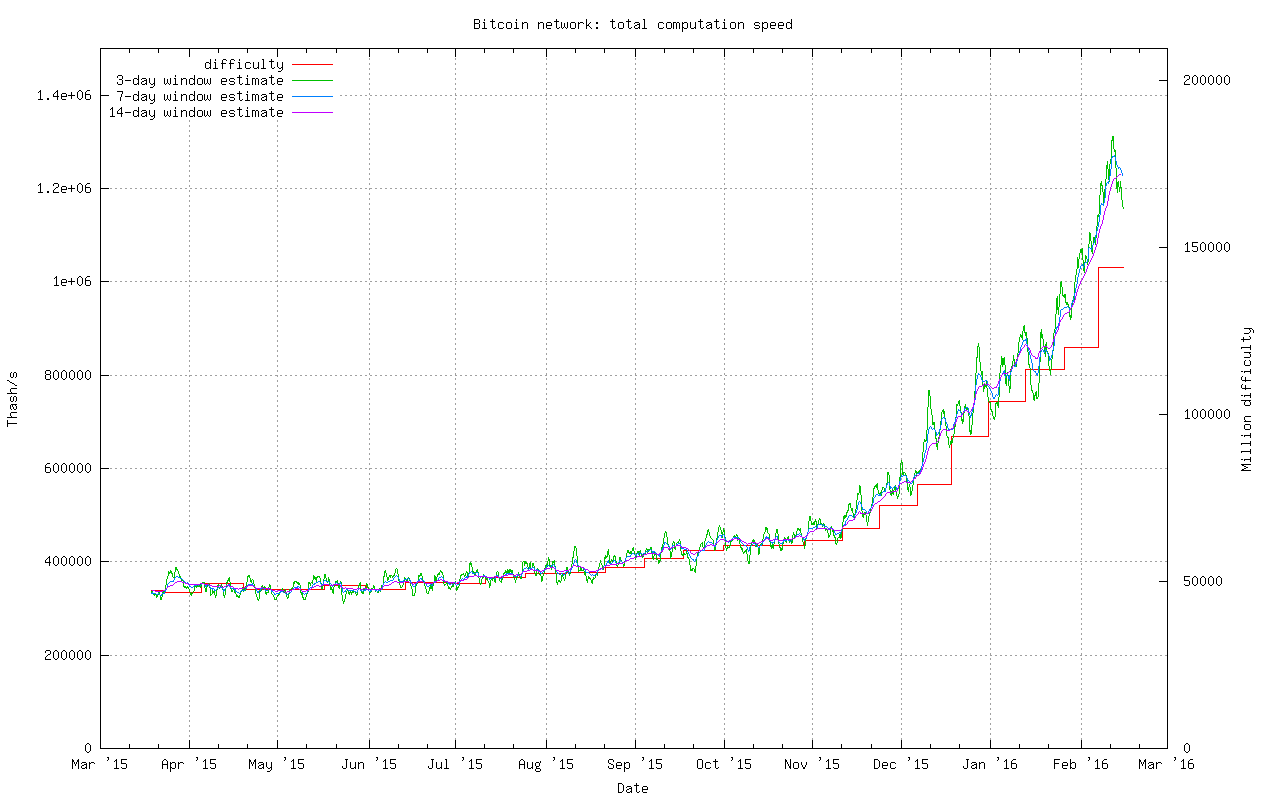
\includegraphics[width=\linewidth]{figs/speed-lin}
		\caption{The computational power of the computers participating in the Bitcoin network, since march of last year, measured in \textbf{trillions} of SHA-256 operations per second \cite{hashing}.  Notice the curve is exponential.   Now glumly consider how much good that would do if it was applied to cancer research.
		   }
		\label{fig:speed-lin}
	\end{figure}
	
	\section{Creating Your Own Nomic Based System}
	
	
	Nomic's initial rules are extremely simple, but allow us to create an incredibly complex systems.
	Likewise, we will present a abstract way to build a Nomic based system.
	
	Implementing a Nomic system can be thought of building 4 different components.
	\begin{itemize}
		\item The \textit{state} of system.  This is the current rules as well as any information needed about participants.
		\item The \textit{Validator}  is  a function which takes in the proposed new block and  returns true or false, depending on whether on not it meets the criteria accepted and executed.
		\item The \textit{Executor} is a function which makes the proposed changes to the the rules and the state of the system.  It also performs any action that needs to be taken independent of the success or failure of a rule change or some other action.
		\item A networking component to communicate with the other members of the system.  We assume updates to the state and proposals are done via pulls.
	\end{itemize}
	
	The first thing is to determine your initial ruleset.
	We recommend that the initial ruleset be built from the ground up using a pure democracy, much like the base rules in Nomic.
	This allows the specific rules for this particular system to be built from the ground up.
	The specific starting rules depend on each use case.
	
	
	\section{Building a Decentralized Identity Management System}
	
	Begin by creating a system of basic rules for management.
	We start by defining which people have power to add new individuals to the system, the \textit{managers}.
	We also need to manage the identities of those who will be managed by the system, which will stored in some data structure denoted as \textit{IDs}.
	
	
	Managers contains the initial list and keys of the entities that have the authority to add new users to the system.
	Managers can add additional managers by voting to add new managers to the system.
	
	IDs, which might names tied to public keys or some unique hash, will also be associated with the manager that added them into the system.
	
	
	
	\section{Building a Blockchain}
	
%	\section{Building a New DNS Service}
	
%	One great advantage over this system is there is modifiable record of whose keys are valid.
	
%	Should a root server become compromised or start issuing invalid keys, the other servers can act and revoke the signer's key, rendering their signed records invalid.
	
	
%	In this scenario, we have two sets of identities stored by Governomic: the DNS records themselves, and those who manage the DNS records.
%	Each root DNS server can autonomously add any DNS record and sign it by with their key.
	
%	What makes the system different from regular DNS is the ability to autorize new 
	
	\section{Auditable And Highly Controlled System}
	
	
	
	
	\section{Addressing Security Concerns}
	The largest problem for security in the system is the ``forking'' problems.
	Suppose you are some new user or you are managing a server that experienced some technical difficulties and lost part of the current chain.
	You pull from your neighbors and discover you
	
	foo \cite{camilleri2010playing}
	 \cite{tezos}
	\bibliography{refs}
	\bibliographystyle{IEEEtran}
\end{document}